\documentclass[conference]{IEEEtran}
\IEEEoverridecommandlockouts
\usepackage{cite}
\usepackage{amsmath,amssymb}
\usepackage{graphicx}
\usepackage{booktabs}
\usepackage{multirow}
\usepackage{url}
\usepackage[hidelinks]{hyperref}
\usepackage{xcolor}
\def\BibTeX{{\rm B\kern-.05em{\sc i\kern-.025em b}\kern-.08em T\kern-.1667em\lower.7ex\hbox{E}\kern-.125emX}}

\begin{document}

\title{LASA-RxGuard: Coupling Handwritten Prescription\\Recognition with Look-Alike/Sound-Alike\\Drug Confusion Risk Flagging}

\author{\IEEEauthorblockN{Tushit Jalan}
\IEEEauthorblockA{\textit{Department of Computer Engineering} \\
\textit{Your College Name}\\
City, India \\
tushit.jalan@gmail.com}
}

\maketitle

\begin{abstract}
Drug names that look or sound alike are a documented cause of dispensing error.
Handwriting removes the orthographic cues that normally separate them, yet
existing work treats recognition and confusion risk as separate problems:
handwriting recognition systems transcribe without assessing danger, and
drug-name confusion research operates on typed names at approval time. We
present LASA-RxGuard, a two-stage system that couples the two. Stage~1 is a
convolutional-recurrent network with CTC loss (8.38M parameters) trained from
scratch on 59{,}000 synthesised handwritten drug-name images. Stage~2 scores the
recognised string against a 2{,}000-name formulary by fusing edit distance,
phonetic encoding and character $n$-gram similarity, and emits a top-3 candidate
list with a three-level risk flag validated against 164 published ISMP/FDA
confusable pairs. On a test split sharing vocabulary and writing style with
training, Stage~1 reaches 2.91\% character error rate (CER), falling to 0.48\%
under lexicon-constrained decoding. We report two negative results that the
evaluation does not support suppressing. First, held-out \emph{vocabulary} costs
almost nothing (2.83\% CER) while held-out \emph{writing style} costs
$6.7\times$ more (19.45\%), indicating that style diversity, not lexicon size,
is the binding constraint. Second, under our visually-biased noise model,
edit distance alone outperforms the three-signal fusion on every metric
measured, so the fusion is not justified by this evaluation. A fine-tuned
transformer baseline failed to converge within the available compute and is
reported as a failed run rather than a comparison.
\end{abstract}

\begin{IEEEkeywords}
handwriting recognition, CTC, medication safety, look-alike sound-alike,
drug-name confusion, patient safety
\end{IEEEkeywords}

\section{Introduction}
Confusing drug names is among the most common causes of medication error
worldwide~\cite{who2007lasa}. Pairs such as \textsc{dop}amine and
\textsc{dobut}amine, or Celebrex and Celexa, are published as known hazards
precisely because clinicians keep confusing them. Orthographic and phonetic
similarity are established risk factors~\cite{lambert1999similarity}, and
mitigations such as Tall Man lettering exploit the visual distinction between
them~\cite{filik2004tallman}.

Handwriting defeats that mitigation. A handwritten prescription has no
controlled capitalisation, and the pharmacist has seconds to decide. Two
research lines address parts of this problem without meeting. Handwriting
recognition~\cite{shi2017crnn,puigcerver2017mdlstm,li2023trocr} reads text
accurately but its benchmarks contain no drug vocabulary and it never asks
whether a confident reading is dangerous. Drug-name confusion
research~\cite{kondrak2006confusable,emmerton2020lasasoftware} measures exactly
that danger, but on typed names at drug-approval time; the FDA's POCA
tool~\cite{fda2009poca} screens proposed names before marketing, not readings
taken at the counter.

This paper couples them. Our contributions are:

\begin{itemize}
\item A two-stage pipeline that carries recognition uncertainty into an
explicit confusion-risk decision, with human-readable justification
(Sections~\ref{sec:stage1}--\ref{sec:stage2}).
\item A reproducible synthesis pipeline producing 59{,}000 handwritten
drug-name images, with an \emph{adversarial split design} that separates
memorisation from generalisation along vocabulary and style axes
independently (Section~\ref{sec:data}).
\item A CTC feasibility analysis showing that na\"ive aspect-preserving
resizing rendered 47.8\% of our training set unable to contribute gradient --
silently, without raising an error (Section~\ref{sec:feasibility}).
\item Honest reporting of two negative results: the style/vocabulary asymmetry,
and the failure of our three-signal fusion to beat edit distance alone
(Sections~\ref{sec:results}--\ref{sec:discussion}).
\end{itemize}

\section{Related Work}
\textbf{Sequence recognition.} Connectionist Temporal Classification
(CTC)~\cite{graves2006ctc} enables training on unsegmented input by marginalising
over alignments, and underpins the CRNN architecture~\cite{shi2017crnn} that
integrates convolutional features, bidirectional recurrence and transcription.
Puigcerver~\cite{puigcerver2017mdlstm} showed one-dimensional BLSTM layers
outperform multidimensional LSTM at lower cost. TrOCR~\cite{li2023trocr}
replaces both with pre-trained transformers, at substantially higher inference
cost.

\textbf{Data.} The IAM database~\cite{marti2002iam} is the standard offline
handwriting benchmark but contains essentially no medication names. Synthetic
generation is well established: elastic distortion~\cite{simard2003elastic} and
synthetic rendering engines~\cite{jaderberg2014synthetic} can substitute for
labelled data, while generative models~\cite{fogel2020scrabblegan} synthesise
handwriting styles directly.

\textbf{Prescription recognition.} Tabassum et al.~\cite{tabassum2022online}
recognise online (stylus) medical words with a BiLSTM, reporting 93.0\% average
accuracy. Pavithiran et al.~\cite{pavithiran2022multilang} target multi-language
prescriptions. Closest to our pipeline, Ali et al.~\cite{ali2024multihead}
combine Mask R-CNN segmentation with TrOCR and hybrid string matching against a
medicine database. Notably, their headline 1.4\% CER is the validation-split
figure; their held-out test split reports 15.44\% before string matching and
13.51\% after -- the same seen/unseen asymmetry we quantify in
Section~\ref{sec:results}. Crucially, all three stop at transcription or
nearest-name matching; none emits a risk judgement.

\textbf{Confusion detection.} Kondrak and Dorr~\cite{kondrak2004identification,
kondrak2006confusable} introduced BI-SIM (orthographic) and ALINE (phonetic)
measures, finding that neither dominates: BI-SIM wins on mixed sets, ALINE on
sound-alike sets. Our ablation revisits this question with a different
conclusion under a different noise model (Section~\ref{sec:discussion}).
Similarity computation rests on edit distance~\cite{levenshtein1966binary},
Jaro-Winkler~\cite{winkler1990string} and Double
Metaphone~\cite{philips2000metaphone}.

\textbf{Alerting.} Clinicians override drug safety alerts in 49--96\% of
cases~\cite{vandersijs2006override}. Any flagging system must therefore be
evaluated on false-positive rate, not recall alone -- a constraint that directly
shaped our threshold calibration.

\section{Dataset Construction}\label{sec:data}

\subsection{Drug-name corpus}
We assembled 2{,}000 drug names from RxNorm~\cite{nlm2024rxnorm} term types
\texttt{IN} (ingredients) and \texttt{BN} (brand names), India's National List
of Essential Medicines~\cite{mohfw2022nlem}, and the names appearing in our
ground-truth pair list. Raw RxNorm \texttt{IN} contains 14{,}648 concepts, most
of which are IUPAC chemical strings or allergenic extracts rather than
prescribable names; we apply a morphological filter and rank survivors by
ground-truth membership, then NLEM membership, then recognised INN stem.

\subsection{Ground truth}
We curated 164 unique confusable pairs covering 272 distinct names from
published ISMP and FDA/ISMP Tall Man material. All 272 names are guaranteed
present in the corpus: a retrieval score against a database missing the ground
truth would be meaningless.

\subsection{Synthesis}
Setting a word in a handwriting font yields uniform letterforms on a straight
baseline, which a convolutional network can exploit. We therefore render
\emph{per glyph}, applying independent baseline wobble, rotation, scale and
spacing, a sinusoidal baseline drift across the word, and explicit cursive
connectors. Degradation then models the imaging path: paper texture, uneven
illumination, ruled lines, ink pressure variation, shear, elastic
distortion~\cite{simard2003elastic}, motion blur, sensor noise and JPEG
artefacts. Twenty-five Open Font License handwriting faces are used, SHA-256
pinned for reproducibility.

A \emph{legibility guard} rejects and redraws any sample whose ink-to-paper
contrast falls below threshold. Without it, aggressive augmentation silently
produces samples no human can read: mislabelled data that caps achievable CER
and teaches the model to guess from word length.

\begin{figure}[t]
\centering
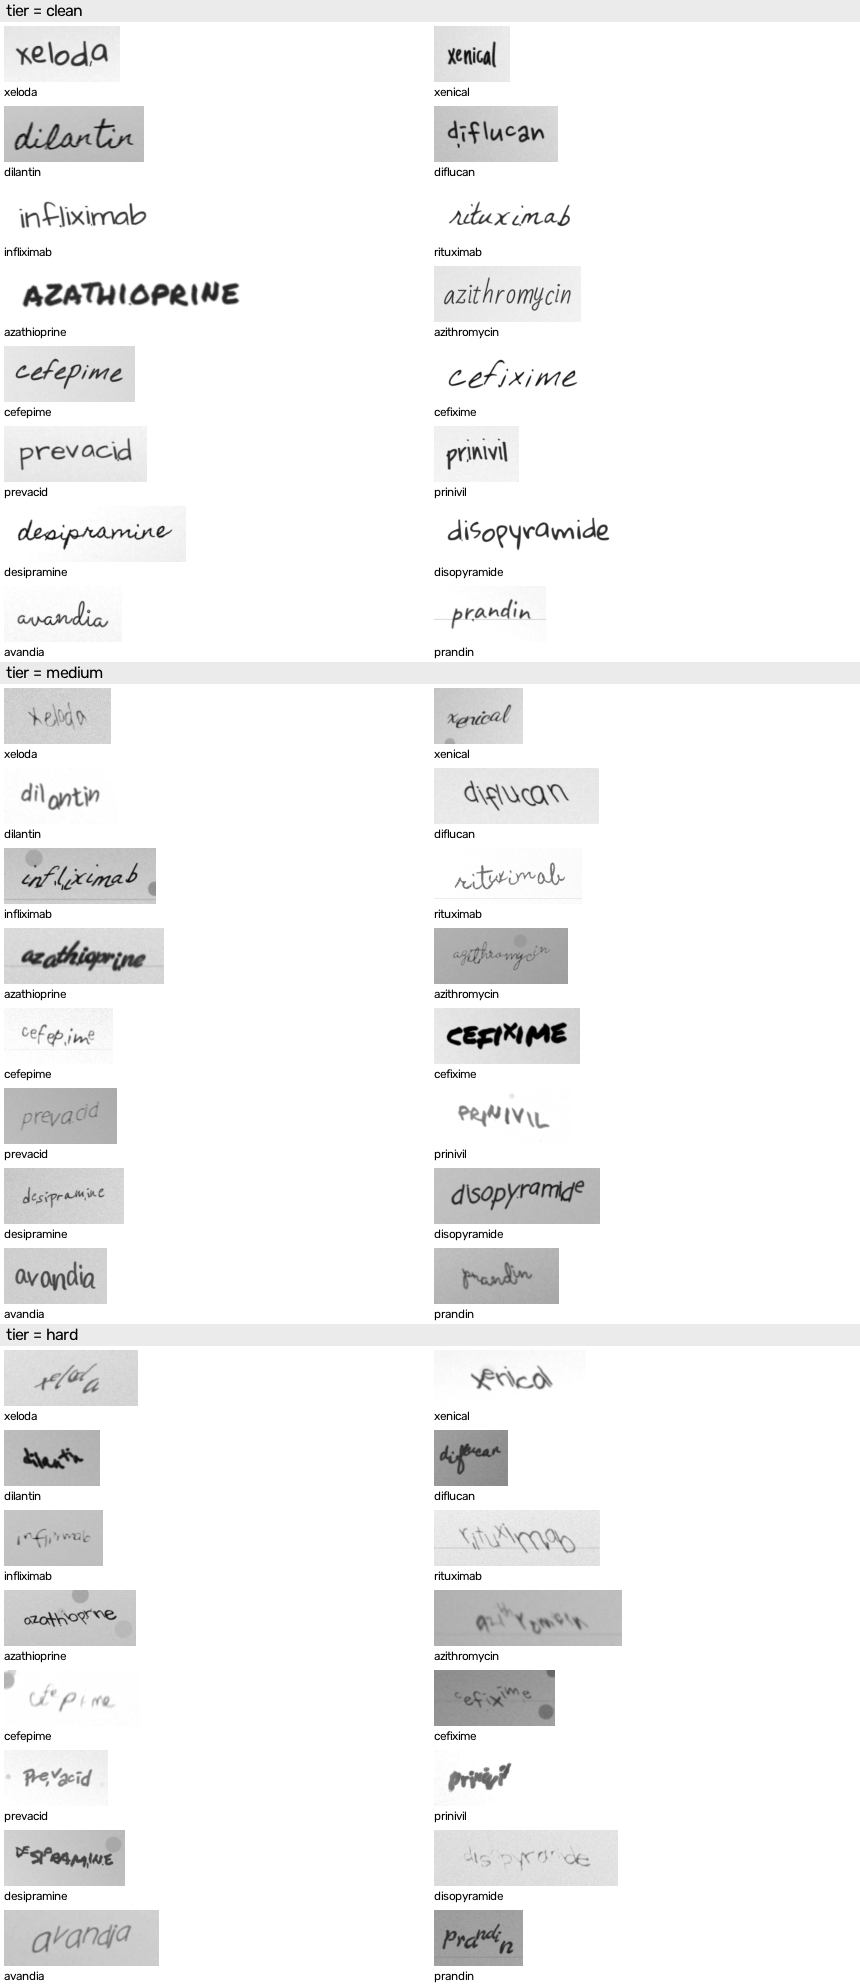
\includegraphics[width=0.72\columnwidth]{figures/synth_preview.png}
\caption{Synthesised samples across three difficulty tiers. Each row shows a
documented confusable pair; ground-truth labels appear beneath.}
\label{fig:synth}
\end{figure}

\subsection{Real handwriting}
We additionally extract word crops from \texttt{Teklia/IAM-line}, a public
mirror of IAM~\cite{marti2002iam}. IAM is line-level, so word boundaries are
inferred from vertical-projection whitespace gaps. A line contributes samples
only when the number of detected crops exactly equals the number of transcript
tokens; otherwise the alignment is a guess that would inject label noise. This
discards 69.1\% of lines, yielding 22{,}506 word images.

\subsection{Adversarial splits}
A single test set cannot distinguish a model that reads from one that memorises.
We hold out vocabulary and writing style on independent axes (Table~\ref{tab:splits}),
with disjointness verified programmatically across the 59{,}000-row manifest.

\begin{table}[t]
\caption{Test splits (names omit the \texttt{test\_} prefix).
Holdouts are seeded and verified disjoint.}
\label{tab:splits}
\centering
\footnotesize
\begin{tabular}{@{}lccp{2.55cm}@{}}
\toprule
Split & Vocab. & Style & Measures \\
\midrule
\texttt{seen}         & train & train & operational accuracy \\
\texttt{unseen\_font} & train & \textbf{held out} & robustness to an unfamiliar hand \\
\texttt{unseen\_word} & \textbf{held out} & train & character-level generalisation \\
\texttt{hard}         & \textbf{held out} & \textbf{held out} & both at once \\
\bottomrule
\end{tabular}
\end{table}

Training uses 48{,}000 images over 1{,}800 words and 20 fonts; 200 words and 5
fonts are held out. Validation uses 3{,}000 images; each test split 2{,}000.

\section{Stage 1: Recognition}\label{sec:stage1}

\subsection{Architecture}
We use a CRNN~\cite{shi2017crnn}: a VGG-style convolutional trunk reducing input
height from 32 to 1 while dividing width by exactly 4, followed by a two-layer
bidirectional LSTM (hidden size 256) and a linear projection to 28 classes
(26 letters plus hyphen plus CTC blank). The model has 8{,}379{,}740 parameters.
Training uses CTC loss~\cite{graves2006ctc} with AdamW and a one-cycle schedule.

\subsection{The CTC feasibility constraint}\label{sec:feasibility}
CTC requires at least $2L+1$ encoder frames to express a label of length $L$,
allowing for blank separators. Samples violating this constraint are not merely
difficult: with \texttt{zero\_infinity} enabled they return zero loss and
\emph{zero gradient}, vanishing from training without raising an error.

Our images are stored at height 64. Aspect-preserving resize to the model height
of 32 halves the width; with the network's $\div4$ width stride, a median
146\,px crop yields only 18 frames for a label requiring 21. Measured over the
training split, \textbf{47.8\% of samples were CTC-infeasible}, and the model
duly collapsed to predicting all blanks --- a failure that presents as a
hyperparameter problem. Applying a horizontal stretch (cancelling the height
reduction) plus a per-sample width floor of $4(2L+1)$ pixels reduces
infeasibility to 0\%, with a median frame slack of 18. We report this because
the failure is silent and, in our experience, easily misattributed.

\subsection{Decoding}
We evaluate three conditions, reported as separate rows throughout: greedy
best-path, prefix beam search ($k=8$), and lexicon-constrained decoding that
snaps output to the nearest of the 2{,}000 known names. The third is the mode a
pharmacy would deploy, since the formulary is fixed and known; it is a different
task from free transcription and is never merged into free-decoding CER.

\section{Stage 2: Confusion Risk Engine}\label{sec:stage2}

\subsection{Similarity signals}
Three signals are computed between the recognised string and each candidate:

\begin{itemize}
\item \textbf{Edit} --- Jaro-Winkler~\cite{winkler1990string} (weight 0.6) and
normalised Damerau-Levenshtein~\cite{levenshtein1966binary} (0.4). Jaro-Winkler
leads because handwriting degrades toward word ends more than beginnings.
\item \textbf{Phonetic} --- Double Metaphone~\cite{philips2000metaphone},
NYSIIS and Soundex codes, compared by similarity rather than equality.
\item \textbf{$n$-gram} --- character trigram TF-IDF cosine, robust to
out-of-vocabulary strings, which OCR output frequently is.
\end{itemize}

These are fused as $s = 0.45\,s_{\text{edit}} + 0.35\,s_{\text{phon}} +
0.20\,s_{\text{ngram}}$.

\subsection{Pair injection}
Documented partners of the top match are force-injected into the candidate list
even when similarity alone would not retrieve them. Candidates carry a
provenance field so that similarity-retrieval and pair-surfacing are reported
separately rather than merged. The system already knows these pairs are
dangerous; failing to surface a published confusable because it ranked fourth
would be indefensible at a dispensing counter.

\subsection{Risk decision}
The traffic light keys off the \emph{ambiguity between the top two candidates},
not the quality of the best match. A confident read of a drug that happens to
have a confusable twin elsewhere in the formulary is not an emergency; an
unresolvable choice between two similar names is. RED fires when the
top two form a documented pair and the reading cannot separate them, or when
similarity exceeds the upper band with a small margin; escalation is automatic
when either drug is ISMP high-alert. YELLOW covers plausible
alternatives and low confidence. A best match below a confidence floor is
reported as \emph{unread}, never GREEN --- an unrecognised string must
not render as safe.

\begin{figure}[t]
\centering
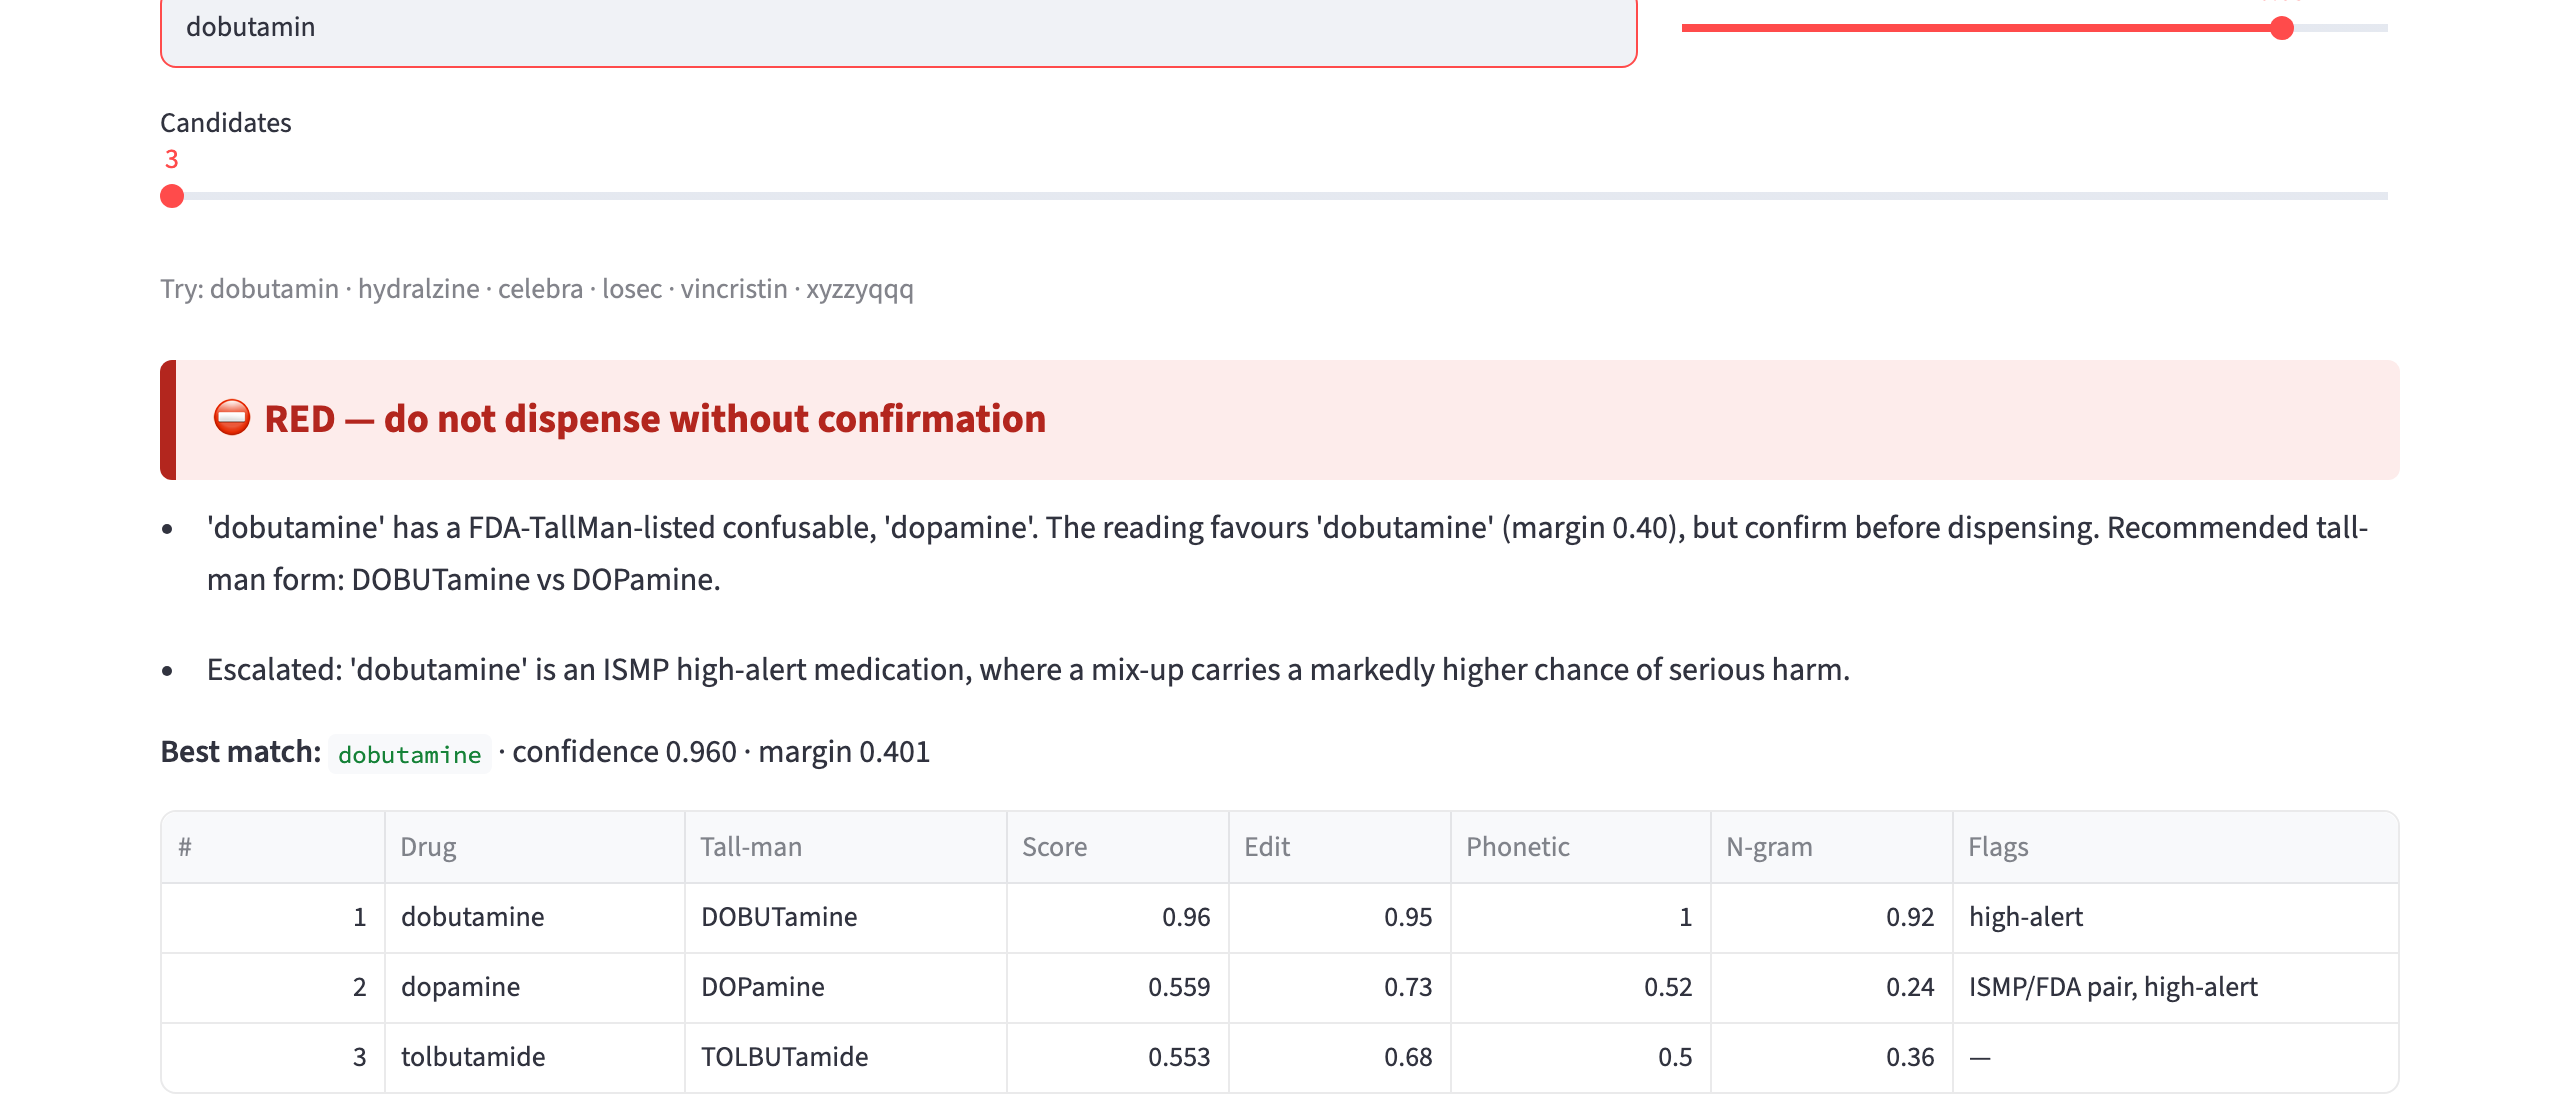
\includegraphics[width=\columnwidth]{figures/demo_red.png}
\caption{System output for the reading \texttt{dobutamin}. The documented
partner \textsc{DOP}amine is surfaced second and the flag escalates to RED
because both drugs are ISMP high-alert. Each alert carries a plain-language
reason and the recommended Tall Man form.}
\label{fig:demo}
\end{figure}

\section{Experimental Setup}
All experiments are seeded (1337); augmentation is baked into stored files so
both model arms train on byte-identical inputs. CER is reported as a
corpus-level micro-average (total edit distance over total reference
characters), not a mean of per-sample rates, which would over-weight short
names. Stage~2 uses a seeded noise model biased toward visually-confusable
substitutions (e.g.\ $a\!\leftrightarrow\!o$, $m\!\leftrightarrow\!n$,
$i\!\leftrightarrow\!l$) with deletion, insertion and transposition.
Hardware: Apple M2 (MPS backend).

\section{Results}\label{sec:results}

\subsection{Stage 1}
Table~\ref{tab:stage1} reports all four splits and three decoders, $n=400$ per
split, from the epoch-5 checkpoint.

\begin{table}[t]
\caption{Stage-1 recognition ($n=400$ per split; split names omit the
\texttt{test\_} prefix). CER/WER lower is better; EM higher is better.}
\label{tab:stage1}
\centering
\footnotesize
\begin{tabular}{@{}llrrr@{}}
\toprule
Decoder & Split & CER & WER & EM \\
\midrule
\multirow{1}{*}{Greedy}
 & \texttt{seen}        & 2.91\%  & 18.25\% & 81.75\% \\
 & \texttt{unseen\_font} & 19.45\% & 70.25\% & 29.75\% \\
 & \texttt{unseen\_word} & 2.83\%  & 19.75\% & 80.25\% \\
 & \texttt{hard}        & 22.71\% & 74.75\% & 25.25\% \\
\midrule
Beam ($k$=8)
 & \texttt{seen}        & 2.80\%  & 17.75\% & 82.25\% \\
 & \texttt{unseen\_font} & 19.09\% & 70.25\% & 29.75\% \\
 & \texttt{unseen\_word} & 2.85\%  & 19.75\% & 80.25\% \\
 & \texttt{hard}        & 22.46\% & 74.50\% & 25.50\% \\
\midrule
Lexicon
 & \texttt{seen}        & \textbf{0.48\%} & 1.25\%  & \textbf{98.75\%} \\
 & \texttt{unseen\_font} & 5.23\%  & 9.00\%  & 91.00\% \\
 & \texttt{unseen\_word} & \textbf{0.08\%} & 0.25\%  & \textbf{99.75\%} \\
 & \texttt{hard}        & 8.16\%  & 13.00\% & 87.00\% \\
\bottomrule
\end{tabular}
\end{table}

Three observations. First, \texttt{test\_unseen\_word} (2.83\%) is
indistinguishable from \texttt{test\_seen} (2.91\%), while
\texttt{test\_unseen\_font} is $6.7\times$ worse: the model learned to read
characters, and \emph{style}, not vocabulary, is the binding constraint.
Second, beam search buys 0.11\,pp of CER for roughly $26\times$ the decode cost
(measured: $<$1\,ms greedy vs 177\,ms beam-10 at batch 32), so greedy is the
correct deployment default. Third, lexicon constraint is transformative but is a
different task.

Error also varies with name length: CER on \texttt{test\_seen} is 6.18\% for
names of 1--6 characters but 0.97\% for names of 15+, since longer names carry
more redundancy for the decoder to exploit.

\subsection{Transformer baseline (failed run)}
We attempted to fine-tune TrOCR~\cite{li2023trocr} as a comparison arm. Within
the available compute --- \texttt{trocr-small-handwritten} (61.6M parameters),
3{,}000 images, 2 epochs, fp32 on MPS at roughly 2 img/s --- validation CER
reached only 96.46\%: the model never left its pre-trained prior. We report this
as a \emph{budget failure, not a verdict on TrOCR}, and draw no conclusion about
the relative merits of the two architectures. A fair comparison requires
\texttt{trocr-base} with fp16 on a CUDA accelerator.

\subsection{Stage 2}
Table~\ref{tab:retrieval} reports retrieval; Table~\ref{tab:flagging} reports
flagging at both operating points, against 164 pairs (both directions) with 300
no-partner controls.

\begin{table}[t]
\caption{Top-$k$ retrieval under simulated OCR noise ($n=400$).}
\label{tab:retrieval}
\centering
\begin{tabular}{@{}rrrr@{}}
\toprule
Errors/char & Top-1 & Top-3 & Top-5 \\
\midrule
0.0 & 98.25\% & 100.00\% & 100.00\% \\
0.1 & 99.00\% & 100.00\% & 100.00\% \\
0.2 & 96.75\% & 99.75\%  & 100.00\% \\
0.3 & 88.50\% & 97.50\%  & 99.75\%  \\
\bottomrule
\end{tabular}
\end{table}

\begin{table}[t]
\caption{Pair flagging. A true positive requires both a flag \emph{and} the
documented partner surfaced. FPR is measured on names with no documented partner.}
\label{tab:flagging}
\centering
\footnotesize
\begin{tabular}{@{}llrrrr@{}}
\toprule
Rule & Err & Prec. & Rec. & F1 & FPR \\
\midrule
RED
 & 0.0 & 100.00\% & 14.33\% & 25.07\% & 0.00\% \\
 & 0.1 & 98.04\%  & 15.24\% & 26.39\% & 0.33\% \\
 & 0.2 & 98.36\%  & 18.29\% & 30.85\% & 0.33\% \\
 & 0.3 & 90.00\%  & 19.21\% & 31.66\% & 2.33\% \\
\midrule
RED+YELLOW
 & 0.0 & 92.11\% & 99.70\% & 95.75\% & 9.33\%  \\
 & 0.1 & 91.85\% & 99.70\% & 95.61\% & 9.67\%  \\
 & 0.2 & 83.81\% & 97.87\% & 90.30\% & 20.67\% \\
 & 0.3 & 65.74\% & 93.60\% & 77.23\% & 53.33\% \\
\bottomrule
\end{tabular}
\end{table}

The two rules bracket a genuine trade-off. RED is a high-precision,
low-recall block-and-confirm gate (98.36\% precision at 0.33\% FPR, 0.2
errors/char). RED+YELLOW is an advisory tier catching 97.87\%
of documented pairs but interrupting 20.67\% of unrelated prescriptions. Given
that clinicians already override 49--96\% of safety
alerts~\cite{vandersijs2006override}, that false-positive rate is itself a
safety concern; we report both rather than only the favourable one.

\subsection{Ablation}
Table~\ref{tab:ablation} isolates each signal at 0.2 errors/char.

\begin{table}[t]
\caption{Signal ablation at 0.2 errors/char ($n=400$). Edit distance alone
outperforms the fusion on every metric.}
\label{tab:ablation}
\centering
\begin{tabular}{@{}lrrr@{}}
\toprule
Configuration & Top-1 & Top-3 & Partner surfaced \\
\midrule
Edit only                   & \textbf{98.75\%} & \textbf{100.00\%} & \textbf{99.70\%} \\
Phonetic only               & 87.00\% & 97.75\%  & 87.50\% \\
$n$-gram only               & 85.25\% & 97.50\%  & 92.38\% \\
Fused (0.45/0.35/0.20)      & 96.75\% & 99.75\%  & 97.87\% \\
\bottomrule
\end{tabular}
\end{table}

\subsection{Deployment envelope}
The CRNN forward pass costs 3.84\,ms mean / 6.79\,ms p95 at batch size 1,
roughly $80\times$ inside a 300\,ms per-word target. Weights are 34\,MB after
stripping optimiser state, with INT8 quantisation~\cite{jacob2018quantization}
expected to reach approximately 8\,MB --- a figure that must be re-measured
rather than assumed, since the dangerous failure mode is not higher CER but a
\emph{confusable} substitution. Decoding, not inference, dominates latency.

\section{Discussion and Limitations}\label{sec:discussion}

\textbf{The fusion is not justified by this evaluation.} Edit distance alone
beats the fused score on top-1, top-3 and partner surfacing
(Table~\ref{tab:ablation}). We retain the phonetic channel on the argument that
our noise model is \emph{biased against it by construction}: it perturbs
characters toward visually-similar glyphs, which is the correct model for OCR
error but systematically rewards orthographic matching. Sound-alike confusion
arises from verbal orders and dictation, an error process we did not
model. Kondrak and Dorr~\cite{kondrak2004identification} found phonetic
measures win precisely on sound-alike test sets. Establishing whether our
phonetic channel earns its weight requires a verbal-error corpus we do not have;
until then, the honest position is that the fusion is unproven here, and a
deployment optimising only for this noise model should use edit distance alone.

\textbf{All handwriting is synthetic.} The gap between degraded font renders and
genuine prescriber handwriting is unmeasured and is the largest single source of
uncertainty in these results. Section~\ref{sec:results} suggests it is
substantial: unseen \emph{fonts} already cost $6.7\times$, and real prescribers
sit further from the training distribution than any held-out font. Generative
handwriting synthesis~\cite{fogel2020scrabblegan} is the most promising route.

\textbf{Other limitations.} The ground-truth pair list is a curated subset of
published ISMP/FDA material, not the complete official table; recall against the
full list is untested. Thresholds are calibrated on a synthetic noise model and
would need recalibration against real OCR error distributions. IAM word crops
are inferred rather than ground-truth segmented, with a 69.1\% discard rate, and
writer-independence could not be verified from the public mirror used. The
transformer arm is unresolved.

\textbf{Not a medical device.} This system has undergone no clinical evaluation
and no prospective study of whether its alerts change dispensing behaviour.
Software supporting clinical decisions falls under CDSCO Medical Device Rules
2017 in India; clinical evaluation, ISO 14971 risk management and IEC 62304
lifecycle process would all precede any deployment. The intended role is
advisory, with a qualified pharmacist making every final decision.

\section{Conclusion}
We presented a two-stage system coupling handwritten drug-name recognition with
explicit look-alike/sound-alike risk flagging, a pairing absent from the
published literature we surveyed. Stage~1 reaches 2.91\% CER on seen conditions
and 0.48\% under lexicon constraint; Stage~2 surfaces 97.87\% of documented
confusable pairs at its advisory operating point. The two findings we consider
most useful are negative: handwriting \emph{style}, not vocabulary, is the
binding constraint on recognition, and our three-signal fusion is not justified
by an evaluation whose noise model is orthographically biased. Future work
should prioritise real prescriber handwriting over model capacity, and a
verbal-error corpus capable of testing the phonetic channel honestly.

\section*{Reproducibility}
Code, the drug corpus, the pair list and all evaluation scripts are available at
\url{https://github.com/TushKum/lasa-rx-guard}. The pipeline is seeded
end-to-end; the 59{,}000-image dataset regenerates byte-identically.

\bibliographystyle{IEEEtran}
\bibliography{references}

\end{document}
